%%
% The BIThesis Template for Bachelor Graduation Thesis
%
% 北京理工大学毕业设计(论文)第二章节 —— 使用 XeLaTeX 编译
%
% Copyright 2020-2023 BITNP
%
% This work may be distributed and/or modified under the
% conditions of the LaTeX Project Public License, either version 1.3
% of this license or (at your option) any later version.
% The latest version of this license is in
%   http://www.latex-project.org/lppl.txt
% and version 1.3 or later is part of all distributions of LaTeX
% version 2005/12/01 or later.
%
% This work has the LPPL maintenance status `maintained'.
%
% The Current Maintainer of this work is Feng Kaiyu.
%%

\chapter{点云配准相关背景知识介绍}
本章将对点云配准的基本理论和相关背景知识进行系统阐述,包括配准的运动学解析、常用数据集、常用配准算法以及相关深度学习方法,并且我们会基于点云配准的评价指标,扩展到多实例点云配准的评价指标。

\section{点云数据}
三维世界中的数据表证有多种类型,如点云数据(Point Clouds)\cite{leberl2010point}、三角网格(Triangle Mesh)\cite{jiang2020local}、体素(Voxel Grids)\cite{guan2020voxel}、深度相机数据(RGB-D Camera)\cite{cruz2012kinect}等,可视化数据如图\ref{fig:3ddata}所示,本文主要研究的是点云数据,因此本节将对点云数据进行简要介绍。

\begin{figure*}[ht]
    \vspace{-8mm}
    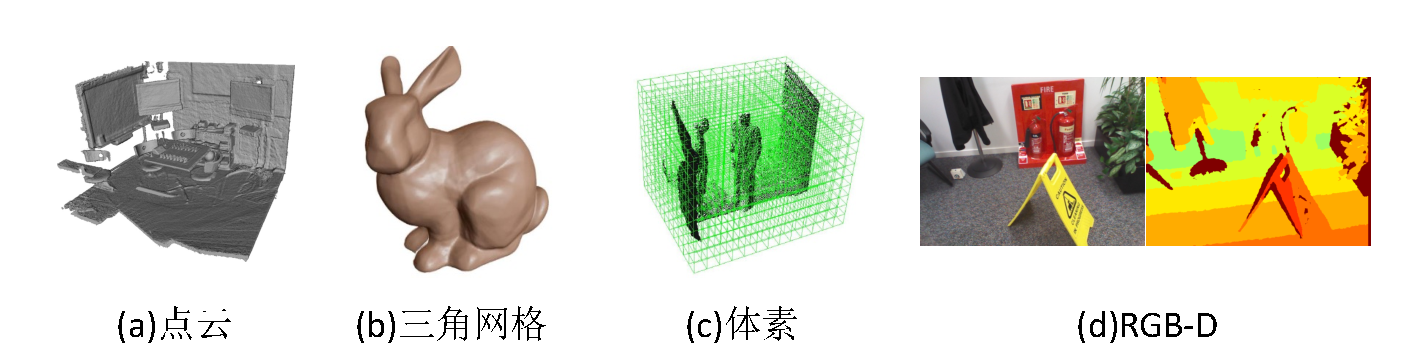
\includegraphics[width=\textwidth]{images/3ddata.pdf}
    \caption{点云、三角网格、体素、深度相机数据可视化示意图}
    \label{fig:3ddata}
    \vspace{-10mm}
\end{figure*}


\subsection{点云数据特点}
点云数据是一种常用的三维数据表征形式,由一系列具有三维坐标(X, Y, Z)的点组成。这些点可以通过激光雷达、结构光传感器、多视角立体视觉等方式采集。点云数据具有以下特点:

1. 无序性:点云数据通常是无序的,即点在数据结构中的顺序并不表示它们在空间中的相对位置。这使得处理点云数据时需要额外关注邻域搜索等问题。

2. 不完整性:由于采集设备的视野限制以及物体遮挡等因素,点云数据往往只能捕捉到物体表面的部分信息,无法完整地描述物体的几何结构。

3. 稀疏性:点云数据在空间中分布可能是不均匀的,有些区域可能点密集,而有些区域可能点稀疏。这会对点云处理算法的性能产生影响。

4. 噪声敏感性:点云数据容易受到测量噪声、环境光照等因素的影响。为了提高数据质量,通常需要对点云进行预处理,如滤波、降采样等。

5. 缺乏拓扑信息:点云数据仅包含物体表面的几何信息,不包含拓扑信息。在需要考虑物体结构的应用场景中,点云数据需要进行进一步处理,如重建三角网格或提取骨架结构等。

6. 可扩展性:点云数据可以方便地扩展以包含其他属性信息,如颜色、法向量、强度等。这有助于提高点云处理算法的性能和鲁棒性。

7. 易于处理和存储:由于点云数据直接表示了物体表面的几何信息,其数据结构简单,便于处理和存储。此外,点云数据可以通过各种数据结构(如KD树、八叉树等)进行高效的组织和检索。

在应用深度学习算法时,由于点云数据的无序性,深度学习算法,比如全连接层、卷积层等无法直接应用于点云数据。因此,需要对点云数据进行预处理,将其转换为有序的数据表征形式,如三角网格\cite{jiang2020local}、体素\cite{guan2020voxel}等。但是这样的方法会造成空间中很多点的浪费,使得输入的数据变得更加稀疏,使得训练数据变少。PointNet\cite{qi2017pointnet}是一种用于处理点云数据的深度学习网络结构,于2017年首次提出。它是一个端到端的神经网络,可以直接从原始点云数据中学习特征表示。PointNet通过使用对称函数(如最大池化)处理输入点云的无序性,同时具有对输入点顺序的不变性。


\subsection{点云特征描述}
三维点云的特征描述,也叫描述子(Descriptor),是一种用于表示点云数据中每个点周围的局部几何特征的向量。描述子捕捉了点云中每个点的几何结构和形状信息,这对于解决诸如点云配准、物体识别、分类和分割等问题至关重要。点云描述子应具有以下特性:鲁棒性、区分性、旋转不变性、尺度不变性和噪声不敏感性。点云描述子对于点云的后处理有着非常巨大的影响,对于不同的任务和数据特征,应该选用合适的描述子来作为网络的预处理。

有许多不同类型的点云描述子,它们根据计算方法和考虑的几何属性而有所不同。以下是一些常见的点云描述子:

1. Spin Images(旋转图像) \cite{johnson1997spin}:通过在点云中每个点周围投影二维图像来表示局部形状信息。

2. Normal Aligned Radial Features(NARF) \cite{steder2010narf}:基于局部表面法线的方向和强度来描述点云中的局部特征。

3. Fast Point Feature Histograms(FPFH) \cite{rusu2009fast}:通过计算每个点周围的点对的几何特征直方图来表示局部特征。

4. Signature of Histograms of Orientations(SHOT) \cite{salti2014shot}:结合局部点的颜色信息和表面法线分布,为每个点计算描述子。

5. Point Pair Features(PPF) \cite{deng2018ppfnet}:描述点云中两个点之间的几何关系,PPF 是一个四元组$(\alpha, d, \theta, \phi)$,其中$\alpha$是两点之间的距离,$d$是两点的法向量之差,$\theta$是两点的法线之间的角度,$\phi$是两点的法线在两点之间连线所确定的平面上的角度。PPF特征在处理点云配准问题时具有很高的鲁棒性,因为它仅依赖于点云的几何信息。

\section{刚体运动参数估计}
刚体运动参数估计是点云配准任务的最后一个阶段的任务。对于位移来说,常用的是位移向量(Transition);旋转的运动参数有不同的表示形式,如欧拉角\cite{pio1966euler}、四元数\cite{shoemake1985animating}、旋转矩阵\cite{horn1954doubly}、轴角\cite{diebel2006representing}等。下面我们对旋转的表示进行简要介绍。

\subsection{欧拉角和轴角}

\subsection{四元数}

\subsection{旋转矩阵}


\subsection{基于SVD的线性代数求解}
\subsection{基于Levenberg-Marquardt算法的非线性优化求解}

\section{标准数据集}
\subsection{ModelNet40}
\subsection{ShapeNet}
\subsection{Scan2CAD}

\section{点云配准评价指标}
\subsection{基于特征提取与匹配的评价指标}
\subsection{基于刚体运动的评价指标}
\subsection{多实例点云配准评价指标}

\section{点云处理与配准相关深度学习技术}
\subsection{深度学习概述}
\subsection{多层感知机}
\subsection{卷积神经网络}
\subsubsection{三维卷积神经网络}
\subsubsection{点云卷积神经网络}
\subsection{注意力机制}
\subsection{谱聚类算法}

\section{小结}

\begin{lstlisting}[language=Python, caption={Python Code}, label={lst:pythonfile}]
import numpy as np

def incmatrix(genl1,genl2):
    m = len(genl1)
    n = len(genl2)
    M = None #to become the incidence matrix
    VT = np.zeros((n*m,1), int)  #dummy variable

    #compute the bitwise xor matrix
    M1 = bitxormatrix(genl1)
    M2 = np.triu(bitxormatrix(genl2),1)

    for i in range(m-1):
        for j in range(i+1, m):
            [r,c] = np.where(M2 == M1[i,j])
            for k in range(len(r)):
                VT[(i)*n + r[k]] = 1;
                VT[(i)*n + c[k]] = 1;
                VT[(j)*n + r[k]] = 1;
                VT[(j)*n + c[k]] = 1;

                if M is None:
                    M = np.copy(VT)
                else:
                    M = np.concatenate((M, VT), 1)

                VT = np.zeros((n*m,1), int)

    return M
\end{lstlisting}
